\documentclass[pdftex,a4paper]{scrartcl}
\usepackage[T1]{fontenc}
\usepackage[utf8]{inputenc}
\usepackage[english]{babel}
\usepackage[final,colorlinks=true,citecolor=blue,linkcolor=black]{hyperref}
\usepackage[babel]{csquotes}
\usepackage[style=numeric]{biblatex}
\usepackage{graphicx}
\usepackage{awesomebox}
\usepackage{dirtree}
%\usepackage{parskip}
\setlength{\parindent}{0px}
\usepackage{lmodern}

\bibliography{latexlit}
%\usepackage[section,nottoc]{tocbibind}

\title{Short Introduction to the Practical-Semester Report Template}
\author{Sebastian Stigler}

\begin{document}

\maketitle

\tableofcontents

\section{\LaTeX{} in General}

\subsection{Where can I get \LaTeX{}?}
\LaTeX{} is distributed in distributions in which the individual packages are bundled so that they fit together.

For Windows, there is either \textbf{\TeX{}Live}\autocite{tug:texlive} or \textbf{MiK\TeX}\footnote{Install in Vista compatibility mode!}\autocite{schenk:miktex}.
MiK\TeX{} should be preferred, because only a relatively small base system is installed and additional packages are then automatically downloaded as needed.

Mac users can use \textbf{Mac\TeX}\autocite{tug:mactex}.

Linux users will usually also find \textbf{\TeX{}Live}\autocite{tug:texlive} as a distribution in their operating system repositories.

\subsection{Which editors can be used?}

In principle, any UTF-8-capable editor can be used. For beginners, it has proven helpful to use editors specifically tailored to \LaTeX{}.

The editor \textbf{\TeX{}maker}\autocite{brachet:texmaker}, available for all operating systems, is definitely recommended.

The editor \textbf{\TeX{}Shop}, which is installed with Mac\TeX{}, is also usable.

In contrast, the editor \textbf{\TeX{}works}, which is installed with MiK\TeX{} and \TeX{}Live, only has very rudimentary features.

\begin{warningblock}
\textbf{UTF-8 and the bibliography}: %
Since the old well-known \texttt{bibtex} program, %
with the help of which \texttt{*.bib} files are prepared %
for the bibliography in \LaTeX{}, does not support UTF-8 %
(and the template already works with the program %
{\texttt{biber}}), in the editors %
the call for the program \textbf{\texttt{bibtex}} %
must be replaced by \textbf{\texttt{biber}}%
\footnote{On Linux, the program must also be installed. %
The package is called \texttt{biber}.}.
\end{warningblock}


\subsection{What about books and reference works?}

As a learning and working book, the book by Joachim Schlosser (Figure~\ref{fig:schlosser}) is recommended. The university library\footnote{From the internal WLAN or from home via VPN.} also provides access to a total of about 11 hours of videos\autocite{schlosser:latex_tutorium} based on this book.

The two classics by Kopka and Mittelbach/Goossens are more suitable as reference works (cf. Figures~\ref{fig:kopka} and \ref{fig:mittelbach_goossens}).

\begin{figure}[h!tbp]
\centering
\begin{minipage}[b]{0.3\textwidth}
\centering

\includegraphics[width=2.5cm]{images/schlosser_latex_buch}
\caption{\autocite{schlosser:latex_buch}}
\label{fig:schlosser}
\end{minipage}
\hfill
\begin{minipage}[b]{0.3\textwidth}
\centering
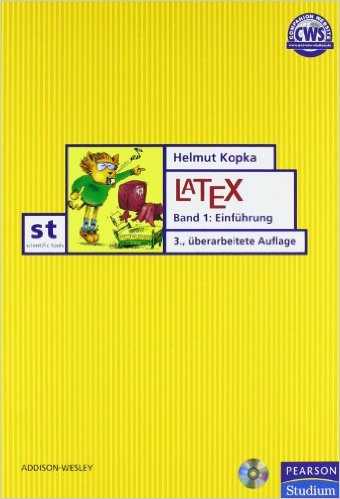
\includegraphics[width=2.5cm]{images/kopka_latex}
\caption{\autocite{kopka:latex}}
\label{fig:kopka}
\end{minipage}
\hfill
\begin{minipage}[b]{0.3\textwidth}
\centering

\includegraphics[width=2.5cm]{images/mittelbach_goossens_latex_begleiter}
\caption{\autocite{mittelbach_goossens:latex_begleiter}}
\label{fig:mittelbach_goossens}
\end{minipage}
\end{figure}

For English-speaking users, I recommend Kottwitz's book\autocite{kottwitz:beginners_guide}.

\clearpage
\section{The Template}

The template consists of the following files:

\dirtree{%
.1 /.
.2 pdf/.
.3 Readme\_DE.pdf\DTcomment{this document in German}.
.3 Readme\_EN.pdf\DTcomment{this document in English}.
.3 TestDokument\_DE.pdf\DTcomment{the compiled sample document in German}.
.3 TestDocument\_EN.pdf\DTcomment{the compiled sample document in English}.
.2 readme/.
.3 images/.
.4 kopka\_latex.jpg.
.4 mittelbach\_goossens\_latex\_begleiter.jpg.
.4 schlosser\_latex\_buch.jpg.
.3 infobox.sty.
.3 latexlit.bib.
.3 Makefile.
.3 Readme\_DE.tex.
.3 Readme\_EN.tex.
.2 vorlage/.
.3 images/.
.4 ausarbeitung.jpg\DTcomment{only for the sample document}.
.4 hs-aalen.jpg.
.3 ausarbeitung.cls.
.3 latexlit.bib.
.3 Makefile.
.3 TestDokument\_DE.tex\DTcomment{the sample document in German}.
.3 TestDocument\_EN.tex\DTcomment{the sample document in English}.
}

To create your own work, please switch to the directory
\texttt{vorlage}.
You can use a copy of \texttt{TestDokument\_DE.tex} or \texttt{TestDokument\_EN.tex}  as a basis.

\subsection{Language}
\label{sec:sprache}

The template is written bilingually.
It is possible to write the paper in either German or English.
At the beginning of \texttt{TestDokument\_*.tex}, the following section is responsible for this:

\begin{verbatim}
%--- Language selection
% Allowed values:
%   \selectlanguage{english}
%   \selectlanguage{ngerman}
\selectlanguage{english}
\end{verbatim}

Simply choose the corresponding language.

The following areas are translated automatically:

\begin{itemize}
  \item Title page
  \begin{itemize}
    \item Document type (practical semester report, project report, bachelor's thesis, seminar paper, master's thesis)
    \item Degree program (Computer Science, Electronics, Data Science)
    \item Transitions between title, company name, and student
    \item Supervisors
    \item Submission date
  \end{itemize}
  \item Company information
  \item Declaration of authorship
  \item Confidentiality clause
  \item Abstract (heading only)
  \item Table of contents, list of figures, list of tables, list of source code, list of abbreviations, and bibliography
  \item The names in the numbering for figures, tables, and source code
\end{itemize}

Everything else must be done by you (chapter headings and content).

\subsection{Title Page}
\label{sec:titleseite}
For the title page, you must use the following commands to adjust the corresponding
entries and generate the title page:

\begin{verbatim}
%--- Type of paper
% Allowed values:
%   \Praxissemesterbericht
%   \Projektbericht
%   \Bachelorarbeit
%   \Seminararbeit
%   \Masterarbeit

\Bachelorarbeit

%--- Degree program:
% Allowed values:
%   \IN % Informatik (Bachelor/Master)
%   \Elektronik
%   \AI % Artificial Intelligence and Data Science (Bachelor)
%   \MLD % Machine Learning and Data Analytics (Master)
\IN

\title{Title of the Paper}

\author{Jon Doe}
\matrikelnr{12345}

%--- Is the first supervisor (\examinerA) at the university a professor?
% Allowed values:
%   \examinerIsAProfessortrue   % Yes
%   \examinerIsAProfessorfalse  % No
\examinerIsAProfessortrue   % Yes

%--- Supervisors
\examinerA{Prof.~Dr.~Rainer~Werthebach}
%\examinerB{Prof.~Dr.~Ulrich~Klauck}

%--- Submission date
\date{20 June 2024}
\end{verbatim}

\begin{warningblock}
\textbf{Something has changed here compared to the old template!}

The type of paper is changed directly using commands such as
\texttt{\textbackslash Bachelorarbeit}, etc.
Please do not forget the backslash!
These commands contain the German and English version of the entry
on the title page.

The same applies to choosing the degree program.

Furthermore, with the commands
\texttt{\textbackslash examinerIsAProfessor\color{blue}true} and
\texttt{\textbackslash examinerIsAProfessor\color{blue}false}, you can now control
whether the text \textit{Supervising Professor} or
\textit{Supervising Staff Member} is shown for the first supervisor.
For the second supervisor, \textit{Second Examiner} is shown on the title page in both cases.
\end{warningblock}

And a bit further down in the document, there is the instruction to display the title page:

\begin{verbatim}
%--- Display title page
\maketitle
\cleardoublepage
\end{verbatim}

\subsection{Company Information}
\label{sec:praxisstelle}
The company must now be described as follows:

\begin{verbatim}
%--- Company information
% Comment out if the paper was not written at an external company.
\companyname{Example Company}
\industrialsector{Example Industry}
\department{Example Department}
\companystreet{Example St. 1}
\companycity{12345 Sample City}

%--- Information about the supervisor at this company
\advisorname{Name of Supervisor}
\advisorphone{(01234) 567-890}
\advisoremail{name@company.xxx}
\end{verbatim}

And a bit further down in the document:

\begin{verbatim}
%--- Display company data
% Comment out if the paper was not written at an external company.
\makeworkplace
\cleardoublepage
\end{verbatim}

\begin{noteblock}
If you are writing your paper (except for the practical-semester report) at the
 university and not at an external company, please comment out both blocks
 using percent signs.
\end{noteblock}

\subsection{Declaration of Authorship and Confirmation}

The declaration and confirmation use the settings
that you made in subsections~\ref{sec:titleseite} and \ref{sec:praxisstelle},
and are generated with the following command:

\begin{verbatim}
%--- Display declaration of authorship
\makeaffirmation
\cleardoublepage
\end{verbatim}

\subsection{Confidentiality Clause}

For external bachelor's or master's theses, it may happen that the paper
contains confidential company data from the company where this paper is written.

After \textbf{consultation with your supervisor at the university}, the paper
can be provided with a confidentiality clause.

\cautionbox{The text of the confidentiality clause is specified by the university

and must not be changed!}

A confidentiality clause can be generated as follows:

\begin{verbatim}
%--- Confidentiality clause (Only works for external bachelor's or master's theses.)
\makeconfidentialclause
\cleardoublepage
\end{verbatim}

\notebox{The confidentiality page is only generated if this is a bachelor's or master's thesis and \texttt{\textbackslash makeworkspace} is enabled.}

\subsection{The Abstract}

Here, the template implements the \verb+abstract+ environment, with which you can write the abstract of your paper:

\begin{verbatim}
\begin{abstract}
  Put the abstract of your paper here.
\end{abstract}
\end{verbatim}


\subsection{Table of Contents, List of Figures, List of Tables, List of Source Code}

Your paper should definitely contain a table of contents (especially since this is done in
\LaTeX{} with one command, \verb+\tableofcontents+).

Depending on your needs, a list of figures, a list of tables, and a list of source code should also be created (provided there are figures or tables in your paper). The following commands are available for this:
\begin{itemize}
  \item \verb+\listoffigures+
  \item \verb+\listoftables+
  \item \verb+\listoflistings+ or \verb+\lstlistoflistings+
\end{itemize}

\notebox{From now on, you can simply leave these commands in the \LaTeX{} document as well. %
The directories are only displayed if they are actually filled with content.}



\subsection{List of Abbreviations}
For the list of abbreviations, the prebuilt document class includes the package
\verb+acronym+. The abbreviations are set in the environment of the same name
and defined with the command \verb+\acro{ReferenceName}[Abbreviation]{LongForm}+:

\begin{verbatim}
\listofabbreviations
\begin{acronym}[Ex.]  % Longest abbreviation in the following
                      % list to determine the width of the column for
                      % abbreviations.

\acro{bsp}[Ex.]{Example}
\end{acronym}
\end{verbatim}

In the text, the abbreviation is then used with \verb+\ac{ReferenceName}+.
When used for the first time, the long form with the abbreviation in parentheses is
printed. For all subsequent uses, only the abbreviation is printed.

\notebox{The \texttt{\textbackslash listofabbreviations} command includes setting a heading (including translation) as well as an entry in the table of contents. Here too, as with
other directories, the list of abbreviations is only displayed if there are
abbreviations defined with \texttt{\textbackslash acro}.}

\subsection{The Remaining Chapters}

You can now use the remaining headings from the sample document as a template for your own paper.

However, if you think that a different structure makes more sense in your case, you are of course free to change this structure.

This may be the case, for example, if you did not receive one large task but many small tasks. Then a chronological description of your activities may be better.

\notebox{If in doubt, consult your supervisor!}


\subsection{The Bibliography}

A bibliography of the sources used is absolutely essential for scientific papers. In \LaTeX{}, this is included via an external file with the extension \verb+.bib+ and the \verb+biber+ tool\footnote{Previously, \texttt{bibtex} was used}.

\notebox{Only entries from the \texttt{.bib} file that were cited also appear in the bibliography! With the \LaTeX{} command \texttt{\textbackslash{}nocite\{...\}}, you can also make entries visible that were not cited.}

In the preamble, you specify with \verb+\bibliography{latexlit}+ that you want to use the file \\\verb+latexlit.bib+. With \verb+\autocite{...}+ you cite an entry in the text, and finally in the appendix you use the command \verb+\printbibliography+ to create the bibliography.

\section{Generating the PDF Document}

If your \LaTeX{} file is called \verb+Praxissemesterbericht.tex+, the following command sequence generates the PDF document:

\begin{verbatim}
pdflatex Praxissemesterbericht.tex
biber Praxissemesterbericht
pdflatex Praxissemesterbericht.tex
pdflatex Praxissemesterbericht.tex
\end{verbatim}

The first call to \texttt{pdflatex} compiles the document, but initially only collects headings, references, and used citations in order to prepare them for use in the corresponding directories and text passages.

From this information, \texttt{biber}, together with the used \texttt{.bib} file, creates the necessary entries for the bibliography and calculates the text markers that should be used for citations in the text.

\textbf{Please note that the \texttt{biber} command only uses the base name of the \texttt{.tex} file \textit{without extension} as its parameter!}

The subsequent \texttt{pdflatex} call now typesets, in addition to the text, the contents of the directories as well as the calculated references, text markers, and citations. However, this may cause the subsequent text to shift due to now longer directories. As a result, the page numbers in these may no longer be correct. For this reason, \texttt{pdflatex} must be called once more.

\appendix
\printbibliography[heading=bibintoc]
\end{document}

%
% EOF
%